%%%%%%%%%%%%%%%%%%%%%%%%%%%%%%%%%%%%%%%%%%%%%%%%%%%%%%%%%%%%%%%%%%%%%%%%%%%%%%%%
% Template for USENIX papers.
%
% History:
%
% - TEMPLATE for Usenix papers, specifically to meet requirements of
%   USENIX '05. originally a template for producing IEEE-format
%   articles using LaTeX. written by Matthew Ward, CS Department,
%   Worcester Polytechnic Institute. adapted by David Beazley for his
%   excellent SWIG paper in Proceedings, Tcl 96. turned into a
%   smartass generic template by De Clarke, with thanks to both the
%   above pioneers. Use at your own risk. Complaints to /dev/null.
%   Make it two column with no page numbering, default is 10 point.
%
% - Munged by Fred Douglis <douglis@research.att.com> 10/97 to
%   separate the .sty file from the LaTeX source template, so that
%   people can more easily include the .sty file into an existing
%   document. Also changed to more closely follow the style guidelines
%   as represented by the Word sample file.
%
% - Note that since 2010, USENIX does not require endnotes. If you
%   want foot of page notes, don't include the endnotes package in the
%   usepackage command, below.
% - This version uses the latex2e styles, not the very ancient 2.09
%   stuff.
%
% - Updated July 2018: Text block size changed from 6.5" to 7"
%
% - Updated Dec 2018 for ATC'19:
%
%   * Revised text to pass HotCRP's auto-formatting check, with
%     hotcrp.settings.submission_form.body_font_size=10pt, and
%     hotcrp.settings.submission_form.line_height=12pt
%
%   * Switched from \endnote-s to \footnote-s to match Usenix's policy.
%
%   * \section* => \begin{abstract} ... \end{abstract}
%
%   * Make template self-contained in terms of bibtex entires, to allow
%     this file to be compiled. (And changing refs style to 'plain'.)
%
%   * Make template self-contained in terms of figures, to
%     allow this file to be compiled. 
%
%   * Added packages for hyperref, embedding fonts, and improving
%     appearance.
%   
%   * Removed outdated text.
%
%%%%%%%%%%%%%%%%%%%%%%%%%%%%%%%%%%%%%%%%%%%%%%%%%%%%%%%%%%%%%%%%%%%%%%%%%%%%%%%%

\documentclass[letterpaper,twocolumn,10pt]{article}
\usepackage{styles}

% to be able to draw some self-contained figs
\usepackage{tikz}
\usepackage{amsmath}

% inlined bib file
\usepackage{filecontents}

%-------------------------------------------------------------------------------
\begin{filecontents}{\jobname.bib}
%-------------------------------------------------------------------------------
@Book{arpachiDusseau18:osbook,
  author =       {Arpaci-Dusseau, Remzi H. and Arpaci-Dusseau Andrea C.},
  title =        {Operating Systems: Three Easy Pieces},
  publisher =    {Arpaci-Dusseau Books, LLC},
  year =         2015,
  edition =      {1.00},
  note =         {\url{http://pages.cs.wisc.edu/~remzi/OSTEP/}}
}
@InProceedings{waldspurger02,
  author =       {Waldspurger, Carl A.},
  title =        {Memory resource management in {VMware ESX} server},
  booktitle =    {USENIX Symposium on Operating System Design and
                  Implementation (OSDI)},
  year =         2002,
  pages =        {181--194},
  note =         {\url{https://www.usenix.org/legacy/event/osdi02/tech/waldspurger/waldspurger.pdf}}}
\end{filecontents}

%-------------------------------------------------------------------------------
\begin{document}
%-------------------------------------------------------------------------------

%don't want date printed
\date{}

% make title bold and 14 pt font (Latex default is non-bold, 16 pt)
\title{\Large \bf Homework 3 Report}

\maketitle

%-------------------------------------------------------------------------------
\section{Introduction}
%-------------------------------------------------------------------------------

The purpose of this assignment was to experiment with the Java Memory Model, or
JMM. The JMM defines how Java programs are able to access shared memory while
avoiding data races. In particular, this assignment was targeted towards the
testing of various synchronization methods used on large arrays of data. These
methods were then measured in terms of real time and CPU time on the lnxsrv06 
and lnxsrv11 servers. Both servers ran Java 15.0.2, but provided different
conditions for testing. lnxsrv06 has a Intel(R) Xeon(R) CPU E5620 @ 2.40GHz,
while lnxsrv11 has a Intel(R) Xeon(R) Silver 4116 CPU @ 2.10GHz. In addition,
lnxsrv06 runs on Red Hat Version 7.8, while lnxsrv11 runs on Red Hat Version 8.2.
Testing was done through the provided \texttt{UnsafeMemory} test harness. In the end, the goal was to achieve
data-race free behavior
while also analyzing potential performance gains compared to the use of the
\texttt{synchronized} keyword.

%-------------------------------------------------------------------------------
\section{AcmeSafeState Implementation}
%-------------------------------------------------------------------------------

Performance-wise, the problem with \texttt{SynchronizedState} was that of locking.
As described in Lea's paper, use of \texttt{synchronized} blocks in the program
results in mutual exclusion of execution. This adds extra overhead to our runtime,
as threads are requried to process Acquire mode reads and Release mode writes in
order to maintain a DRF state. As seen in all tests run on \texttt{SynchronizedState},
this extra overhead resulted in a worse runtime when compared to single-thread
execution:

\begin{verbatim}
  Single-thread:
  Total time 2.99502 s real, 2.99319 s CPU
  Multi-threading:
  Total time 28.4691 s real, 91.4220 s CPU
\end{verbatim}

While these results are pulled from a specific test case, the same jump in runtime was
found for all test cases. When the \texttt{synchronized} keyword is removed from
the program, the runtime improves, but the program becomes extremely vulnerable to
race conditions, which is why we need to implement \texttt{AcmeSafeState} as an
alternative method to maintaining DRF. Instead of using \texttt{synchronized} blocks,
\texttt{AcmeSafeState} uses the \texttt{java.util.concurrent.atomic} package. More
specifically, it makes use of the \texttt{AtomicLongArray} class implemented by the
package. According to Lea, this class defines methods based around the VarHandle 
constructions in JDK 9. These methods, including \texttt{getAndDecrement()} and 
\texttt{getAndIncrement()}, which were used to implement the \texttt{swap()} function
of \texttt{AcmeSafeState}, are applied to individual elements of the 
\texttt{AtomicLongArray}. By using these methods instead of traditional increments
and decrements, each operation becomes atomic. This means that it is impossible for them
 to be interrupted like in the race conditions generated by
\texttt{UnsynchronizedState}. At the same time, we avoid the locking behavior that
dominates the runtime of \texttt{SynchronizedState}, deferring to VarHandles-based
structures instead in order to maintain DRF. 

%-------------------------------------------------------------------------------
\section{Obstacles}
%-------------------------------------------------------------------------------

The largest obstacle I ran into when collecting data on my classes was the
inconsistency of the Linux servers. Since these servers are available to many
students, the load on each server varies greatly over time. As a result, they do
not necessarily offer a stable testing environment. To account for this, I did
my best to record data for all my classes in as little time as possible to
minimize these potential variances. However, this methodology means that I only
ran a single test for each test case. Admittedly, this makes my method vulnerable
to possible outliers that would have been caught with repeated trials. However,
I decided that the benefits of running my tests in a stable environment 
outweighed the possible downsides of outlier cases, especially since many test cases
were used in the first place. Other than that, my data collection process went 
smoothly, although manually testing and recording data did become tedious, so, if I
were to repeat these tests, I would attempt to automate them in some way.

%-------------------------------------------------------------------------------
\section{Measurements and Analysis}
%-------------------------------------------------------------------------------

\begin{figure}
  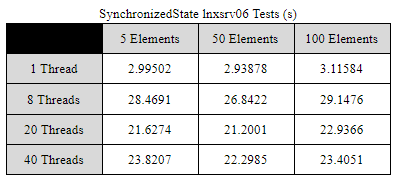
\includegraphics[scale=0.8]{synchronized-06.png}
  \caption{\label{fig:vectors} Table of total time results from testing SynchronizedState on lnxsrv06, measured in seconds. }
\end{figure}

\begin{figure}
  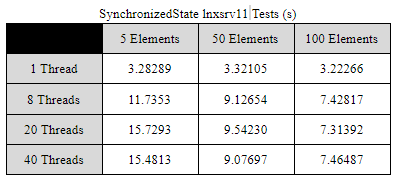
\includegraphics[scale=0.8]{synchronized-11.png}
  \caption{\label{fig:vectors} Table of total time results from testing SynchronizedState on lnxsrv11, measured in seconds. }
\end{figure}

\par The first measurements that were taken over the course of this assignment were
the test cases for the \texttt{SynchronizedState} class. To keep consistency, 
100,000,000 swaps were performed for all tests, but the number of threads used 
for multi-threading varied between 1, 8, 20, and 40, while the array size varied 
between 5, 50, and 100. The provided \texttt{UnsafeMemory} test harness
outputs multiple time measurements, including real time, system CPU time, and user
CPU time. However, these times tended to follow the same trends as the test cases
were varied, so this analysis will focus on the total time to simplify things.
After running tests on \texttt{SynchronizedState}, I proceeded to run the same
test cases on the \texttt{AcmeSafeState} class. Each set of test cases were
performed across the lnxsrv06 and lnxsrv11 servers in order to detect changes
across different hardware implementations. The results of these test cases
are pictured above. 

\begin{figure}
  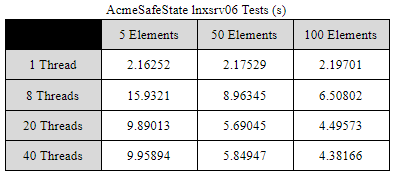
\includegraphics[scale=0.8]{acmesafe-06.png}
  \caption{\label{fig:vectors} Table of total time results from testing AcmeSafeState on lnxsrv06, measured in seconds. }
\end{figure}

\begin{figure}
  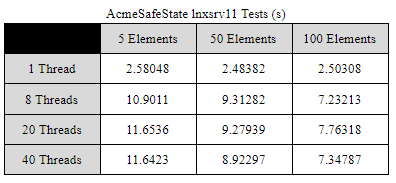
\includegraphics[scale=0.8]{acmesafe-11.png}
  \caption{\label{fig:vectors} Table of total time results from testing AcmeSafeState on lnxsrv11, measured in seconds. }
\end{figure}

\par The first thing that stands out is that, regardless of the synchronization
technique used, the single-threaded execution is always the most efficient in
terms of runtime. This shows that \texttt{SwapTest} is not well suited for
parallelism. It's likely too simple of an operation to gain much benefit from
multi-threading, resulting in the added overhead of multi-threading hurting the
runtime more than it helps. As threads are added, a trend appears where the runtime
spikes at 8 threads, and proceeds to improve as 20 and 40 are tested. This is likely
because the additional threads begin to negate the overhead generated from multi-threading,
resulting in worse runtimes being found at low thread counts. 
\par Another simple conclusion to make focuses on the single-threaded tests.
For both the \texttt{SynchronizedState} and \texttt{AcmeSafeState} classes,
the single-threaded tests ran faster on lnxsrv06 than on lnxsrv11. This seems
to make sense, as lnxsrv06 has more cache memory, which would result in more caching and faster
memory accesses over the course of the testing. Of course, any of the other
differences in the hardware of the servers may also contribute to this difference,
but they would be out of the scope of my knowledge.
\par It is also possible to see that the increase in array size helps performance. This is
because, for both classes, when an array entry is being operated on, it cannot be accessed
by other threads. For this reason, in small arrays, most of the entries will be locked
at any given time, preventing threads from being useful. As the array size is increased
the rate at which these collisions happen will go down, resulting in more efficient processing.
This is true of both synchronization techniques used in this assignment, so both classes
operate more efficiently on large arrays.
\par When looking at the results of \texttt{SynchronizedState}, it's clear that
the use of \texttt{synchronized} blocks was much more effective on lnxsrv11 than
on lnxsrv06. This is despite the single-threaded tests running slower on lnxsrv11
than lnxsrv06. Together, these results seem to point to the conclusion that lnxsrv11
is more suited for taking advantage of multi-threading. However, when looking at
the \texttt{AcmeSafeState} results, the opposite seems to be true. While the differences
are not as drastic as the ones present in the \texttt{SynchronizedState} tests,
running the test harness on lnxsrv06 does seem to produce better runtimes across the
board. The only exception to this is the 5 element, 8 thread case, however, it is likely
that this result is simply a result of the inconsistency of the Linux servers. With
these results in mind, it is perhaps more accurate to say that lnxsrv11 is better suited
for parallelism by way of locking, while lnxsrv06 is better suited for the VarHandle style
of synchronization used by \texttt{java.util.concurrent.atomic}.
\par Continuing on with that conclusion, it is also possible to see this trend when
examining the benefits obtained from using \texttt{AcmeSafeState} over \texttt{SynchronizedState}.
On lnxsrv06, the benefits gained from \texttt{AcmeSafeState} were very large, with runtimes
going down dramatically. However, on lnxsrv11, this is not the case. The benefits gained on
lnxsrv11 are negligible at best. With the inconsistency of the servers, it is impossible
to say whether any benefits actually exist at all. Once again, this points to the
conclusion that lnxsrv06 is much better suited for the parallel behavior exploited by
\texttt{AcmeSafeState}.
\par In summary, the \texttt{SynchronizedState} class seems to work best on lnxsrv11, while the 
\texttt{AcmeSafeState} class seems to work best on lnxsrv06. Both classes benefit greatly from
larger array sizes, and, while single-thread execution is most efficient, multi-threaded
execution is improved as threads are added. Overall, the \texttt{AcmeSafeState} class has
superior performance to the \texttt{SynchronizedState} class in the vast majority of the
tests used here, while maintaining the same degree of reliability.

%-------------------------------------------------------------------------------
\section{References}
%-------------------------------------------------------------------------------
"Package java.util.concurrent.atomic." 
Available: \\ https://docs.oracle.com/en/java/javase/15/docs/api/index.html \\
\\
D. Lea "Using JDK 9 Memory Order Modes." 
Updated November 16, 2018.
Available: \\ http://gee.cs.oswego.edu/dl/html/j9mm.html \\
\\
P. Eggert "Homework 3. Java shared memory performance races." 
Updated January 28, 2021. 
Available: \\ https://web.cs.ucla.edu/classes/winter21/cs131/hw/hw3.html


%%%%%%%%%%%%%%%%%%%%%%%%%%%%%%%%%%%%%%%%%%%%%%%%%%%%%%%%%%%%%%%%%%%%%%%%%%%%%%%%
\end{document}
%%%%%%%%%%%%%%%%%%%%%%%%%%%%%%%%%%%%%%%%%%%%%%%%%%%%%%%%%%%%%%%%%%%%%%%%%%%%%%%%

%%  LocalWords:  endnotes includegraphics fread ptr nobj noindent
%%  LocalWords:  pdflatex acks
